\begin{enumerate}[label=\arabic*.,ref=\thesection.\theenumi]
\numberwithin{equation}{enumi}
\item The modulated signal is given by 
\begin{align}
	s(t) = \cos\brak{2\pi f_c t + \phi(t)}
\end{align}
where
\begin{align}
	\phi(t) = 2\pi k_f \int_{0}^{t}m(\tau)\,d\tau
\end{align}
List the various parameters in a table.
\\
\solution 
\item Obtain a difference equation for computing $\phi(t)$.  Suggest a sampling rate.
\item Plot the spectrum of the transmitted signal.
\\
\begin{figure}[h]
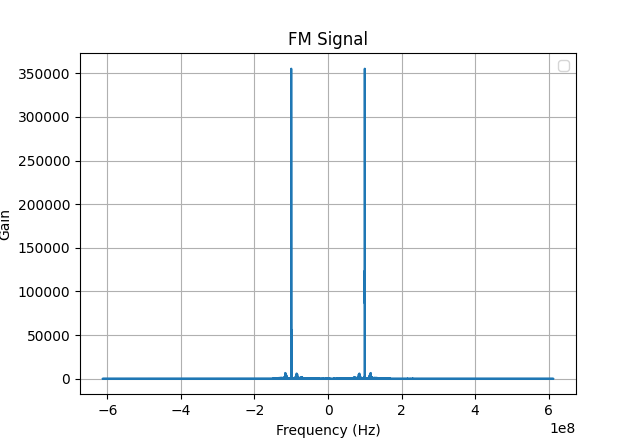
\includegraphics[scale=0.7]{fm/tx/fm.png} 
\end{figure}

\item Compute the bandwidth of the transmitted signal.
\\
\solution Calculate the bandwidth of the transmitted signal by computing the Fourier Transform:
\begin{equation}
S_k = \sum_{n=0}^{N-1} s(n) e^{-j2\pi kn/N}, \quad k=0,1,\dots,N-1
\end{equation}
In code for computing the FFT of s(n)
\begin{equation}
S_k = \texttt{fft}(s(n), N)
\end{equation}
Where $S_k$ is the frequency representation of the signal, s(n) is the transmitted signal. 
we need to calculate its power spectral density. This can be done using the equation \eqref{eq:psd}

Calculating the Power Spectral Density: 
\begin{align}
PSD(s)=\lvert S_k \rvert^2 
\label{eq:psd}
\end{align}
Identify the frequency range with significant power using a mask function.code is given below\\
\begin{center}
\fcolorbox{red}{white}{\parbox{7.5cm}
{\href{https://github.com/KrishnaYadati/signal-processing/tree/main/fm/codes/mod.py}
{/codes/mod.py}}}
\end{center}
\end{enumerate}
